
\chapter{Modelagem FrameWeb}
\label{sec-frameweb}
\vspace{-1cm}

\emph{\imprimirtitulo} é um sistema Web cuja arquitetura utiliza \textit{frameworks} comuns no desenvolvimento para esta plataforma. Desta forma, o sistema pode ser modelado utilizando a abordagem FrameWeb~\cite{souza-celebratingfalbo20}.


\begin{footnotesize}
	\begin{longtable}{|c|c|}
		\caption{\textit{Frameworks} da arquitetura do sistema separados por categoria.}
		\label{tabela-frameworks}\\\hline
		
		\rowcolor{lightgray}
		\textbf{Categoria de \textit{Framework}} & \textbf{\textit{Framework} Utilizado} \\\hline 
		\endfirsthead
		\hline
		\rowcolor{lightgray}
		\textbf{Categoria de \textit{Framework}} & \textbf{\textit{Framework} Utilizado} \\\hline 
		\endhead

		Controlador Frontal & Angular \\\hline

		Injeção de Dependências & Spring Boot (via Spring IoC Container) e Go (\textit{vanilla}) \\\hline

		Mapeamento Objeto/Relacional & Spring Boot (Spring Data JPA) e Go (pgx) \\\hline

        Mapeamento Objeto/Documento & Spring Boot (Spring Data MongoDB) e Go (mongo-driver) \\\hline

		Segurança & Spring Boot (via Spring Security) \\\hline
	\end{longtable}
\end{footnotesize}

A Tabela~\ref{tabela-frameworks} indica os \textit{frameworks} presentes na arquitetura do sistema que se encaixam em cada uma das categorias de \textit{frameworks} que FrameWeb dá suporte. Em seguida, os modelos FrameWeb são apresentados para cada camada da arquitetura. Para isso, foram selecionadas algumas funcionalidades para serem representadas nos modelos, as quais são:
\begin{itemize}
    \item a funcionalidade de cadastro e autenticação;
    \item a funcionalidade de buscas das repúblicas, incluindo possibilidade de filtros diversos;
    \item a funcionalidade de gerência das repúblicas dos locadores.
\end{itemize}

\section{Camada de Negócio}
\label{sec-frameweb-negocio}

A camada de negócio é responsável pelas regras de negócio do sistema e possui os pacotes \textbf{Application} e \textbf{Domain}, que são representados pelos modelos de \textbf{Entidade} e de \textbf{Aplicação}.

\subsection{Modelo de Entidades}

O modelo de entidade apresenta os objetos de domínio e suas relações \cite{phdthesis}. Especificamente para o sistema \emph{\imprimirtitulo}, as classes \textbf{Crib}, \textbf{Review}, \textbf{Location}, \textbf{Image} e \textbf{User}, que pode ser \textbf{Tenant} ou \textbf{Landlord}, integram esse modelo, como pode ser visto na Figura~\ref{figura-arquitetura-entidades}. 

Um \textbf{Crib} é o objeto que representa uma república dentro do sistema. Ele contém um \textbf{Location}, que é a entidade responsável por armazenar os dados relacionados às coordenadas. Um \textbf{Crib} pode conter vários \textbf{Reviews}, que são as entidades responsáveis por armazenar os comentários públicos que os moradores, chamados de \textbf{Tenant} no sistema, deixam juntamente com seu \emph{rating}, um valor numérico equivalente a estrelas, como em plataformas como o \textit{Airbnb}~\footnote{https://www.airbnb.com}. O usuário do tipo \textbf{Landlord}, que é o locador dentro do sistema, ao cadastrar um \textbf{Crib}, pode adicionar imagens para que os potenciais moradores tenham uma noção de como é o local por dentro.

\begin{figure}[h]
	\centering
	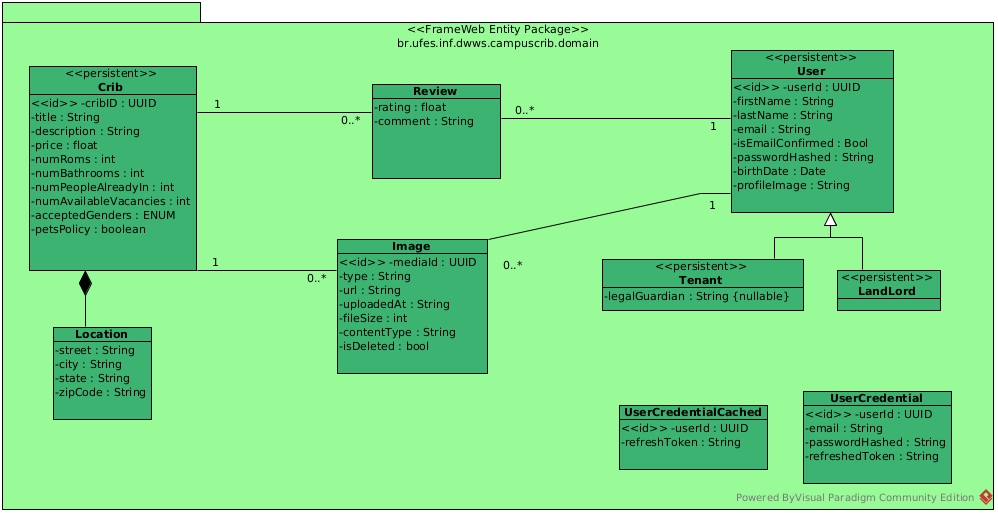
\includegraphics[width=0.8\textwidth]{figuras/modelo-de-entidades.jpg}
	\caption{Modelo de Entidades}
	\label{figura-arquitetura-entidades}
\end{figure}

No modelo de entidade, é possível observar duas entidades que possuem o prefixo \textbf{User}, mas que não apresentam o comportamento de um usuário convencional. Essas entidades existem para representar as informações armazenadas no fluxo de autenticação e autorização. \textbf{UserCredential} representa as credenciais de autenticação de um usuário para a autenticação no padrão JWT~\footnote{https://jwt.io}. O \textbf{UserCredentialCached} é a entidade de cache da credencial de um usuário, em que  o objetivo é de armazenar, em um banco apropriado para cache de dados, um usuário que foi logado recentemente, evitando assim muitas chamadas ao banco de dados que contêm as credenciais.

\subsection{Modelo de Aplicação}

O modelo de aplicação é onde ficam as classes de serviço \cite{phdthesis} e onde ocorre a implementação das funcionalidades e regras de negócio. No modelo, é possível ver as classes controladoras e suas dependências, que são as classes de serviço e as classes de persistência (DAO). 

No sistema \emph{\imprimirtitulo}, adicionamos às interfaces dos serviços o sufixo UseCase para representar a granularidade das operações, que são chamadas em rotas diferentes. Por exemplo, a interface \textbf{CribManagerUseCase}, que representa o serviço \textbf{CribManagerService}. Além de gerenciar a criação e atualização dos Cribs, esse serviço também interage com outros módulos do sistema, como o \textbf{CribSearch}, por meio do método \textbf{sendMessageToCribSearch}. Esse método utiliza um message broker (Kafka) para direcionar as mensagens conforme a necessidade do sistema.


\begin{figure}[h]
\centering
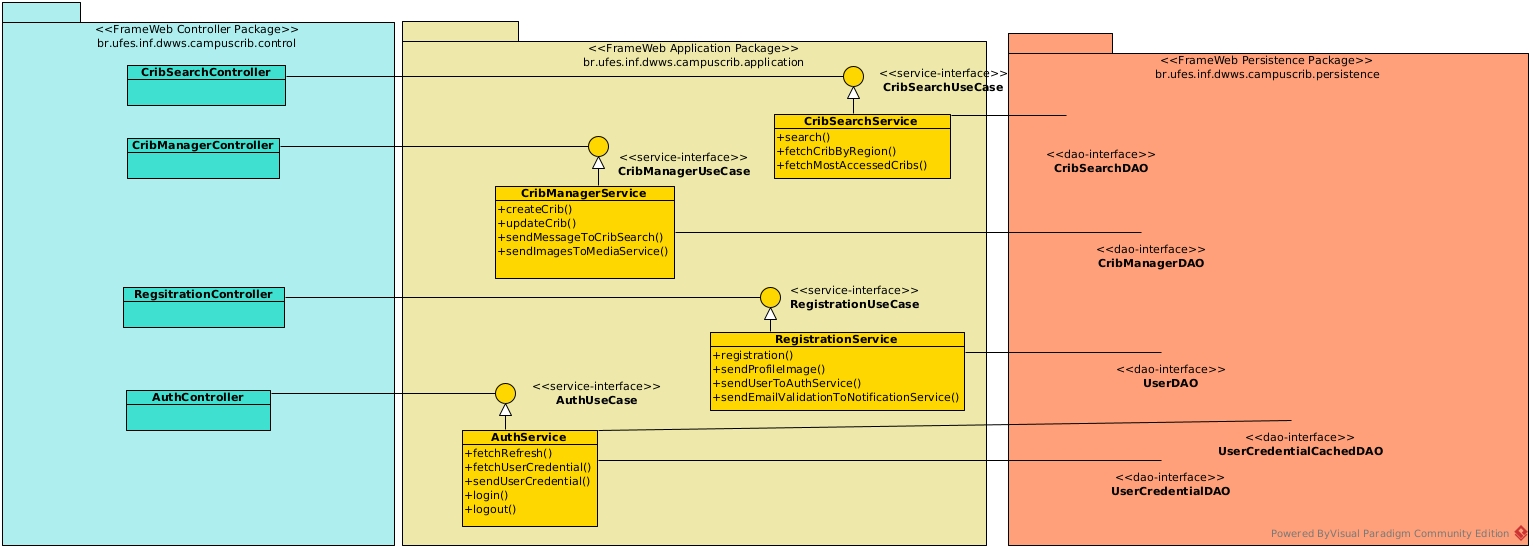
\includegraphics[width=0.8\textwidth]{figuras/modelo-de-aplicacao.jpg}
\caption{Modelo de Aplicação}
\label{figura-arquitetura-aplicacao}
\end{figure}

A figura~\ref{figura-arquitetura-aplicacao} apresenta o modelo de aplicação, em que no centro está (em amarelo) o pacote de aplicação com os serviços e as suas interfaces (casos de uso). A esquerda (em ciano) se tem o pacote control com os controladores em que utilizam os serviços via os casos de uso. A direita (em vermelho) está o pacote de persistência apresentando as interfaces DAO, que são utilizadas pelos serviços.


\section{Camada de Acesso a Dados}
\label{sec-frameweb-dados}

A camada de Acesso a Dados é responsável por gerenciar o armazenamento e a recuperação dos dados do sistema \cite{phdthesis}. Nessa camada, são definidos os repositórios e os objetos que representam as entidades persistidas no banco de dados, garantindo a comunicação entre a aplicação e a base de dados de forma organizada e eficiente.


\subsection{Modelo de Persistência}

O modelo de persistência representa os objetos responsáveis por armazenar os dados gerados pelo sistema. Seguindo o padrão de abstração DAO, esse modelo centraliza todas as interações com o banco de dados, que ocorrem por meio do ORM \cite{phdthesis}.

Os repositórios \textbf{CribSearchDAO}, \textbf{CribManagerDAO} e \textbf{UserCredentialCachedDAO} são interfaces responsáveis pela persistência dos dados relacionados às funcionalidades do sistema \emph{\imprimirtitulo}. O \textbf{CribSearchDAO} é utilizado para a indexação e busca de \emph{Cribs}, enquanto o \textbf{CribManagerDAO} trata da criação, edição e gerenciamento dos \emph{Cribs}, além de contemplar as interações entre usuários e os processos relacionados às propostas. O \textbf{UserCredentialDAO} gerencia as credenciais de acesso dos usuários no sistema e o \textbf{UserCredentialCachedDAO} gerencia as credenciais em cache.

O objeto \textbf{UserDAO} representa a interface de persistência dos dados dos usuários no sistema. Ele contempla todas as operações básicas de criação, atualização, leitura e deleção, bem como funcionalidades específicas associadas aos perfis de \emph{Tenant} e \emph{Landlord} dentro da plataforma.

\begin{figure}[h]
	\centering
	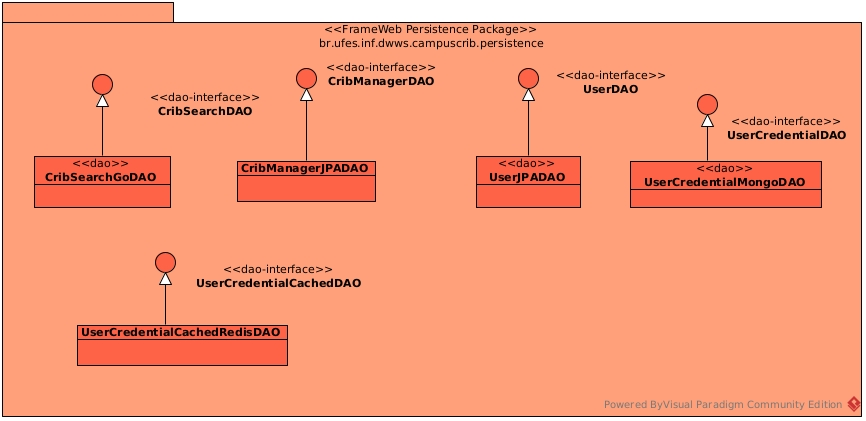
\includegraphics[width=0.8\textwidth]{figuras/modelo-de-persistencia.jpg}
	\caption{Modelo de Persistência}
	\label{figura-arquitetura-persistencia}
\end{figure}

A Figura~\ref{figura-arquitetura-persistencia} apresenta o modelo de persistência do \emph{\imprimirtitulo}, conforme as interfaces supracitadas. Cada uma das interfaces DAO possuem suas implementações, que na figura aparecem relacionadas as interfaces por generalização. Como há diferentes bancos de dados, bem como diferentes linguagens para os microsserviços, então, em \textit{camel case}, a última palavra antes de DAO apresenta qual ORM ou forma de implementar a interface é utilizado. Por exemplo, temos: \textbf{CribSearchGoDAO} implementa \textit{CribSearchDAO} em Go; já \textbf{CribManagerJPADAO} implementa via \textit{JPA} a interface \textit{CribManagerDAO}; para o cache, tem-se \textbf{UserCredentialCachedRedisDAO} implementando a interface \textit{UserCredentialCachedDAO}.


\section{Camada de Apresentação}
\label{sec-frameweb-apresentacao}

A camada de apresentação \cite{phdthesis} é responsável pela parte da aplicação que faz a interface com o usuário, e os modelos de navegação servem para guiar e mapear como será a experiência do usuário com a aplicação.


\subsection{Modelo de navegação Crib Manager}

O modelo de navegação do Crib Manager é o modelo que mostra o processo de gerenciamento dos Cribs dentro do sistema.  
O \textbf{CribManager} é responsável por interagir com os usuários do sistema, criação e atualização do Crib, sendo a parte de gestão das repúblicas de um usuário locador.  

\begin{figure}[h]
	\centering
	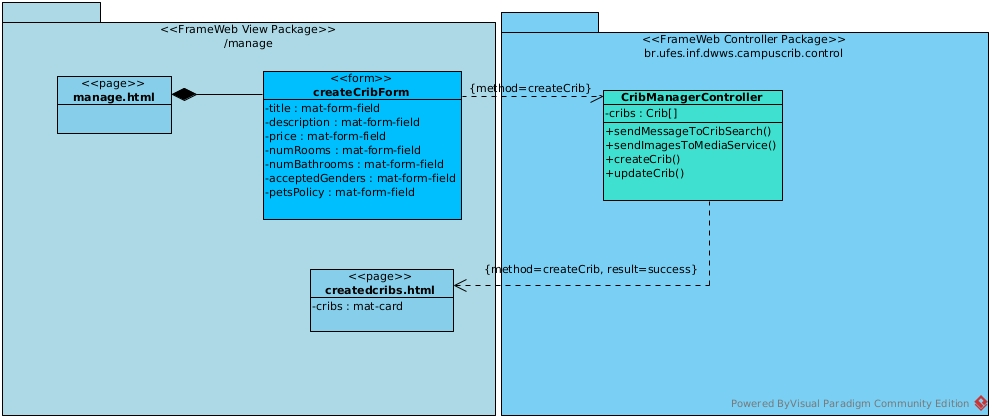
\includegraphics[width=0.8\textwidth]{figuras/modelo-de-navegacao-crib-manager.jpg}
	\caption{Modelo de Navegação Crib Manager}
	\label{figura-arquitetura-nav-crib-manager}
\end{figure}

A figura~\ref{figura-arquitetura-nav-crib-manager} apresenta o modelo de navegação do Crib Manager, em que para o cadastro e edição de uma república tem-se um formulário para enviar os dados da república para o controlador \textbf{CribManagerController}, que retorna as repúblicas do locador, em que são apresentadas por \textit{cards} do Angular Material.

\subsection{Modelo de navegação Crib Search}

O modelo de navegação \textbf{Crib Search}, apresentado na figura~\ref{figura-arquitetura-nav-crib-search}, é o modelo que mostra o processo de busca no sistema. A busca é feita através de um componente \textbf{mat-field} no \textit{front-end}, que gerencia o \textit{input} digitado e o autocomplete para gerar a \textit{query} de busca. A busca pode ser feita por diversos critérios, como por região, que usa a geolocalização informada. Inicialmente, o filtro utilizado é de localização do navegador do usuário atual e, com isso, são trazidos os Cribs que respeitam as condições solicitadas. Os Cribs são mostrados na página através do componente \textbf{mat-card}, que renderiza um Crib e seus dados cadastrados pelo locador (\textbf{Landlord}).

\begin{figure}[h]
	\centering
	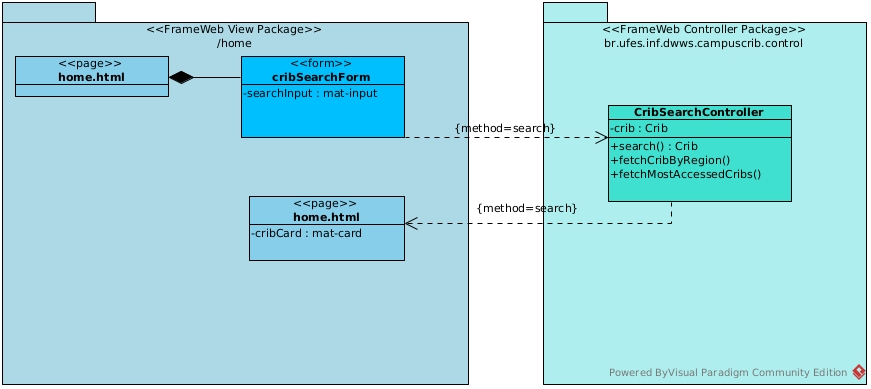
\includegraphics[width=0.8\textwidth]{figuras/modelo-de-navegacao-crib-search.jpg}
	\caption{Modelo de Navegação Crib Search}
	\label{figura-arquitetura-nav-crib-search}
\end{figure}

\subsection{Modelo de navegação Registration/Auth}

O modelo de navegação \textbf{Registration/Auth}, apresentado na figura~\ref{figura-arquitetura-nav-registration-auth}, é um modelo que mostra o processo de criação do usuário e autenticação, que não são dois processos separados, mas complementares dentro do sistema. A criação é feita pelo \textbf{Registration}, que no \textit{front-end} são componentes \textbf{Angular} e um formulário que é enviado para o \textit{back-end}. A camada de controle para nós é a camada de controle do \textit{back-end}. A parte do controlador e serviços do \textit{front-end} são abstraídos no nosso modelo. Essas requisições vão para um \textit{gateway} em que serão direcionadas para o \textbf{Registration Service} (microsserviço responsável pela criação e onde o controlador se encontra).

\begin{figure}[h]
	\centering
	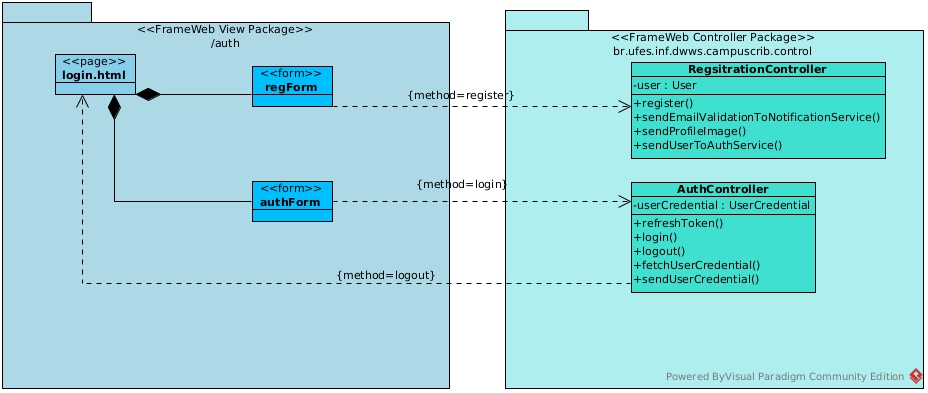
\includegraphics[width=0.8\textwidth]{figuras/modelo-de-navegacao-registration-auth.jpg}
	\caption{Modelo de Navegação Registration/Auth}
	\label{figura-arquitetura-nav-registration-auth}
\end{figure}

Já a parte do login, chamada de \textbf{Auth}, que realiza a autorização e autenticação do usuário, segue o mesmo padrão do \textbf{Registration}, mas também fica responsável pela criação e gerenciamento das credenciais dos usuários do sistema através do padrão JWT.
